\section{Expected signal}
We present in this section the calculation of the expected signal. The
main ingredients are:
\begin{itemize}
\item the sun flux (the sun flux varies with time)
\item the sun path with respect to the antenna depending on the time of the year
\item the antenna pattern
\end{itemize}
Given these  ingredients can then  calculate the expected  increase of
power collected output by the antenna and deduce the expected increase
of the baseline for a given system temperature.

\subsection{Sun flux}
In our frequency range ~ GHz,  the sun flux has two main contributions
~\cite{solarflux}:  a quiet  sun component  (or  background component)
with a constant intensity and a frequency dependence as:
\begin{equation} 
 Sq \  [SFU] =  26.4 +  12.4 \ \nu  + 1.11\  \nu^2 \\ \rm  for \  (1 <
 \nu(GHz) < 20)
\end{equation}
a    second    contribution,   the    so    called   slowly    varying
component, its spectrum is parameterised as:
\begin{equation}
    Sv  \ [SFU]= \frac{0.64 ( F10.7 - 70 ) f^{0.4}}{ 1 + 1.56 ( ln \ ( \ f  \ / \  2.9 ) )^2}
\end{equation}
These spectra are shown in the figure~\ref{fig:spectra}
\begin{figure}[!ht]
  \centering
  \hspace*{-3ex}
  \subfigure{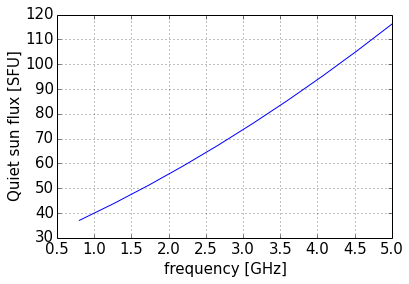
\includegraphics[width=0.49\linewidth]{quietsunspec.png}}
  \subfigure{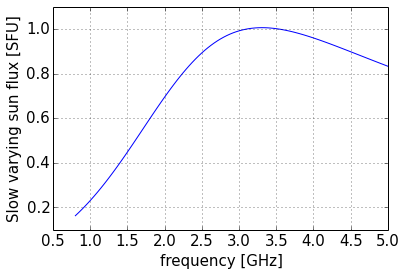
\includegraphics[width=0.49\linewidth]{varyingsunspec.png}}
  \caption{Left: quiet sun spectrum, Right: varying component spectrum}
  \label{fig:spectra}
\end{figure}
The  intensity of  the total  flux at  2.8GHz (F10.7)  is  measured by
several  observatories\cite{nobeyamaobs}, \cite{nasa}.  Making  use of
these data  and the parameterization  in frequency written  above, one
can deduce the flux in the C-band.


\paragraph{F10.7}
\begin{figure}[!ht]
  \centering
  \hspace*{-3ex}
  \subfigure{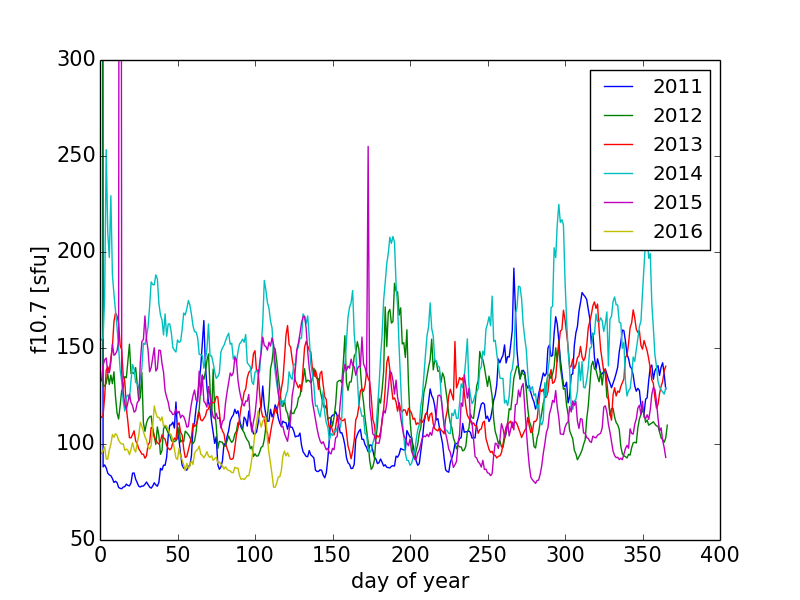
\includegraphics[width=0.7\linewidth]{f10_72011_2016.png}}
  \caption{Left: quiet sun spectrum, Right: varying component spectrum}
  \label{fig:spectra}
\end{figure}


\paragraph{sun path}
\begin{figure}[!ht]
  \centering
  \hspace*{-3ex}
  \subfigure{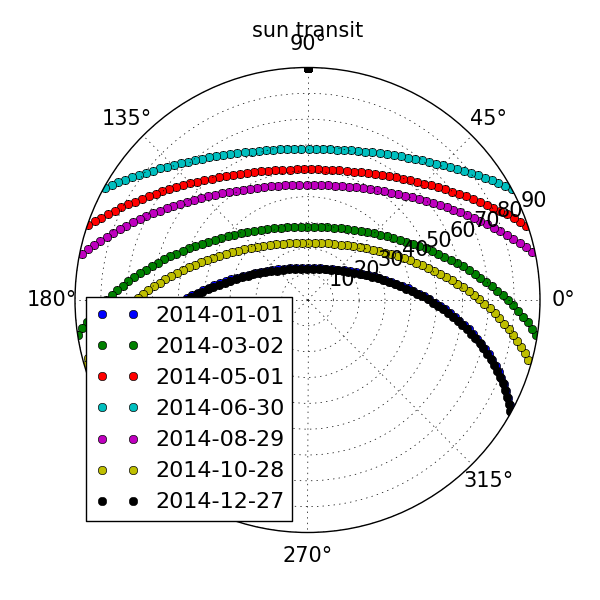
\includegraphics[width=0.7\linewidth]{sunpath.png}}
  \caption{Left: quiet sun spectrum, Right: varying component spectrum}
  \label{fig:spectra}
\end{figure}

\paragraph{expected signal}
\begin{figure}[!ht]
  \centering
  \hspace*{-3ex}
  \subfigure{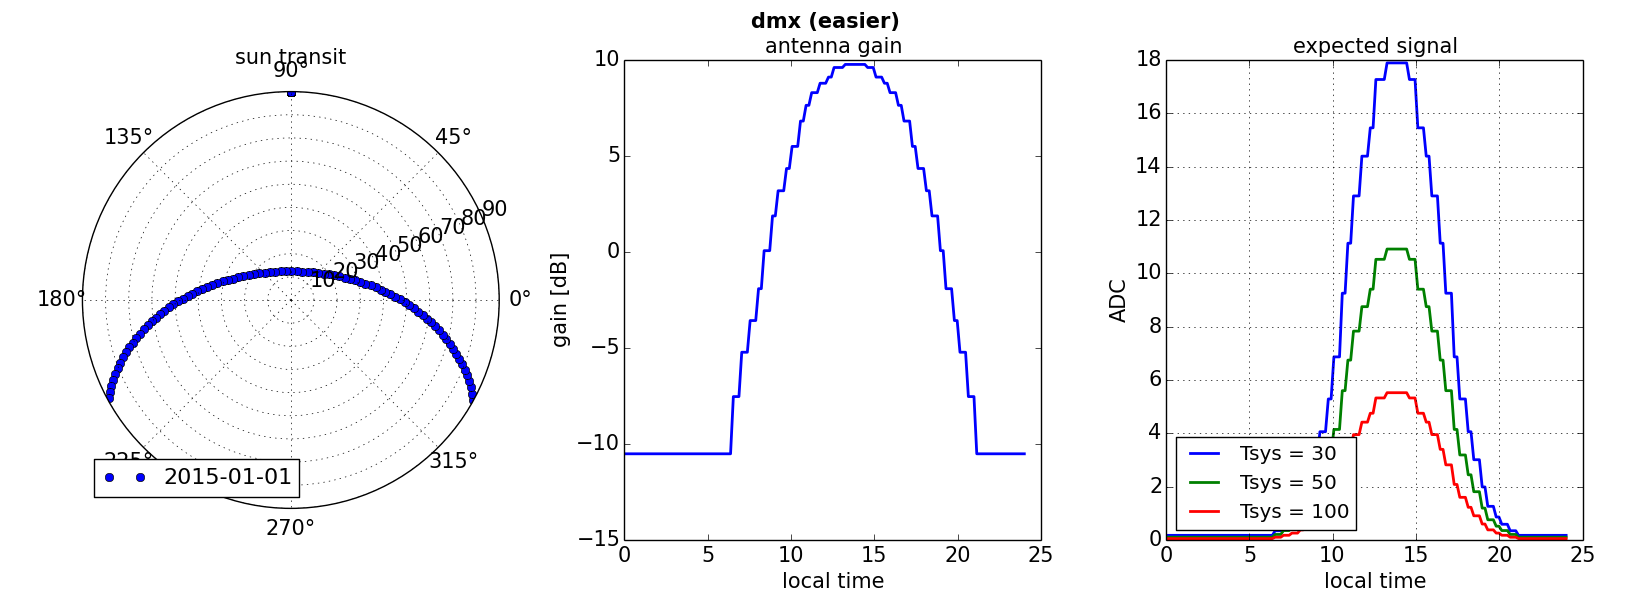
\includegraphics[width=0.7\linewidth]{expeasier.png}}\\
  \subfigure{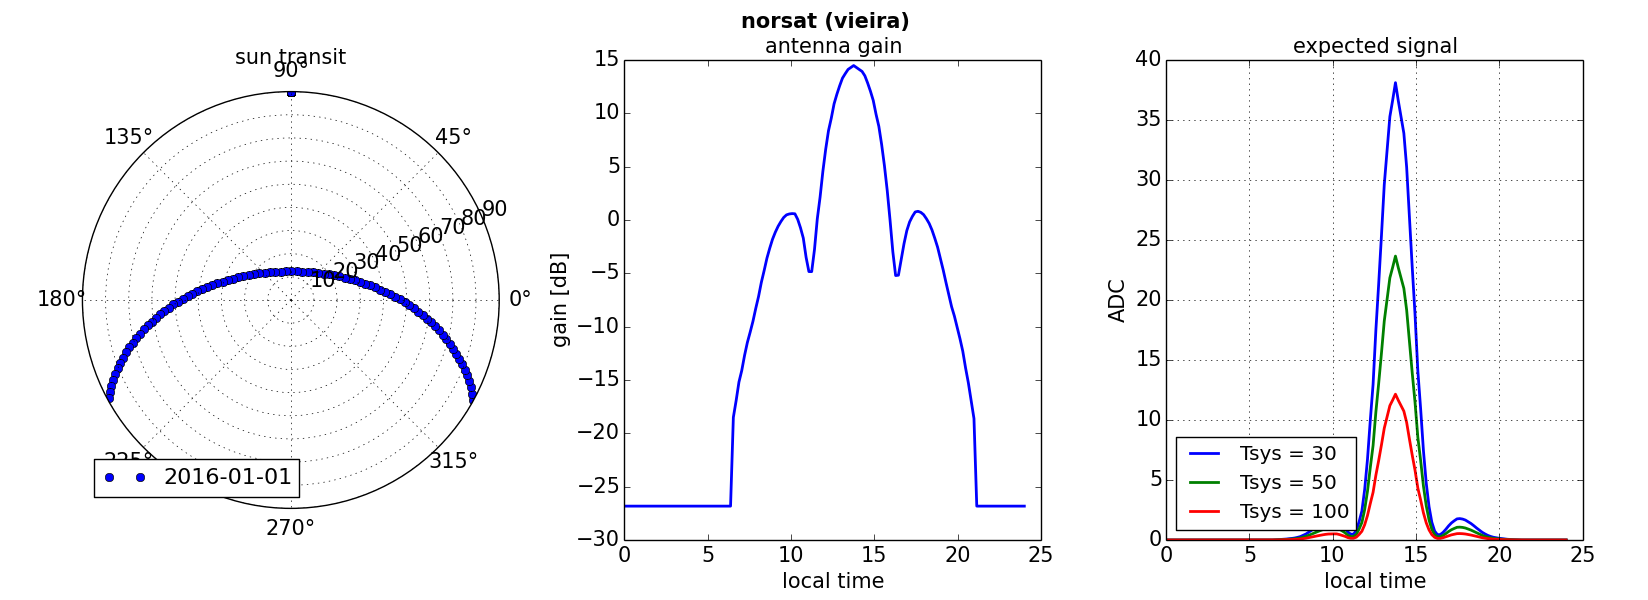
\includegraphics[width=0.7\linewidth]{expvieira20160101.png}}\\
  \subfigure{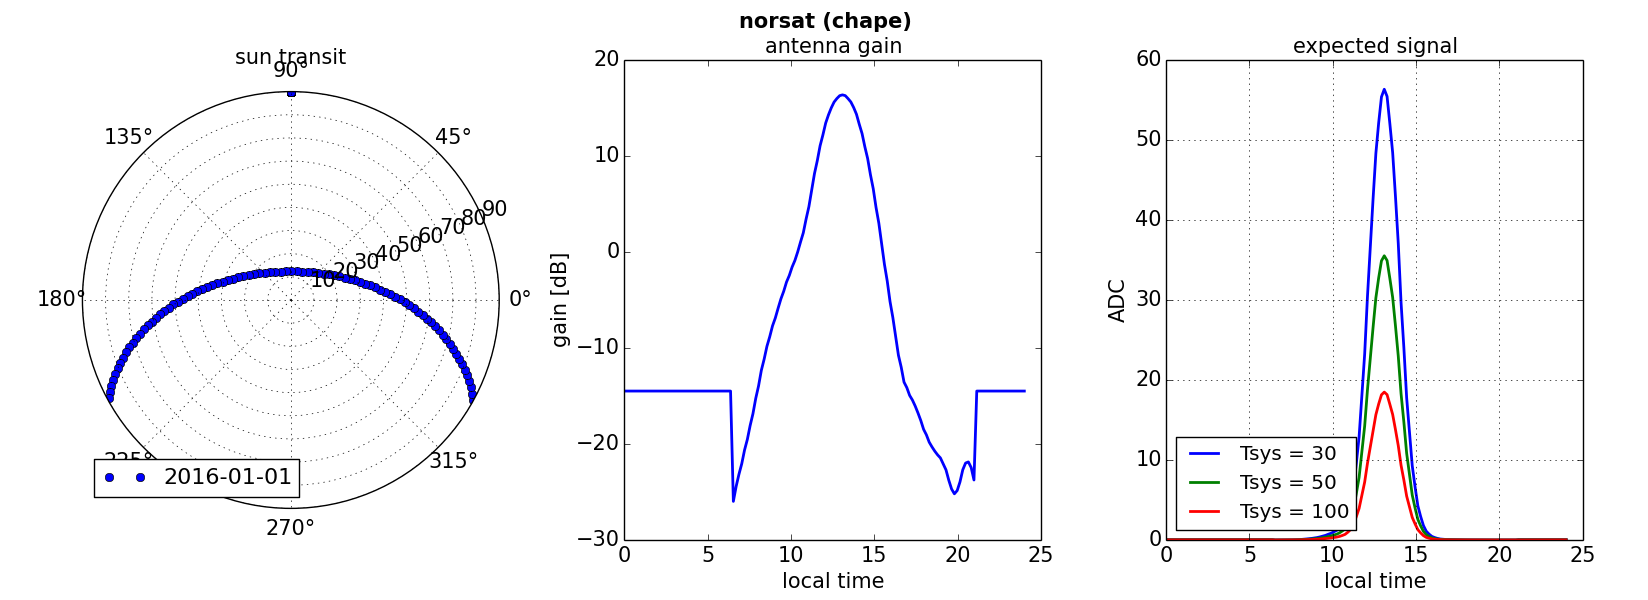
\includegraphics[width=0.7\linewidth]{expchape20160101.png}}\\
  \subfigure{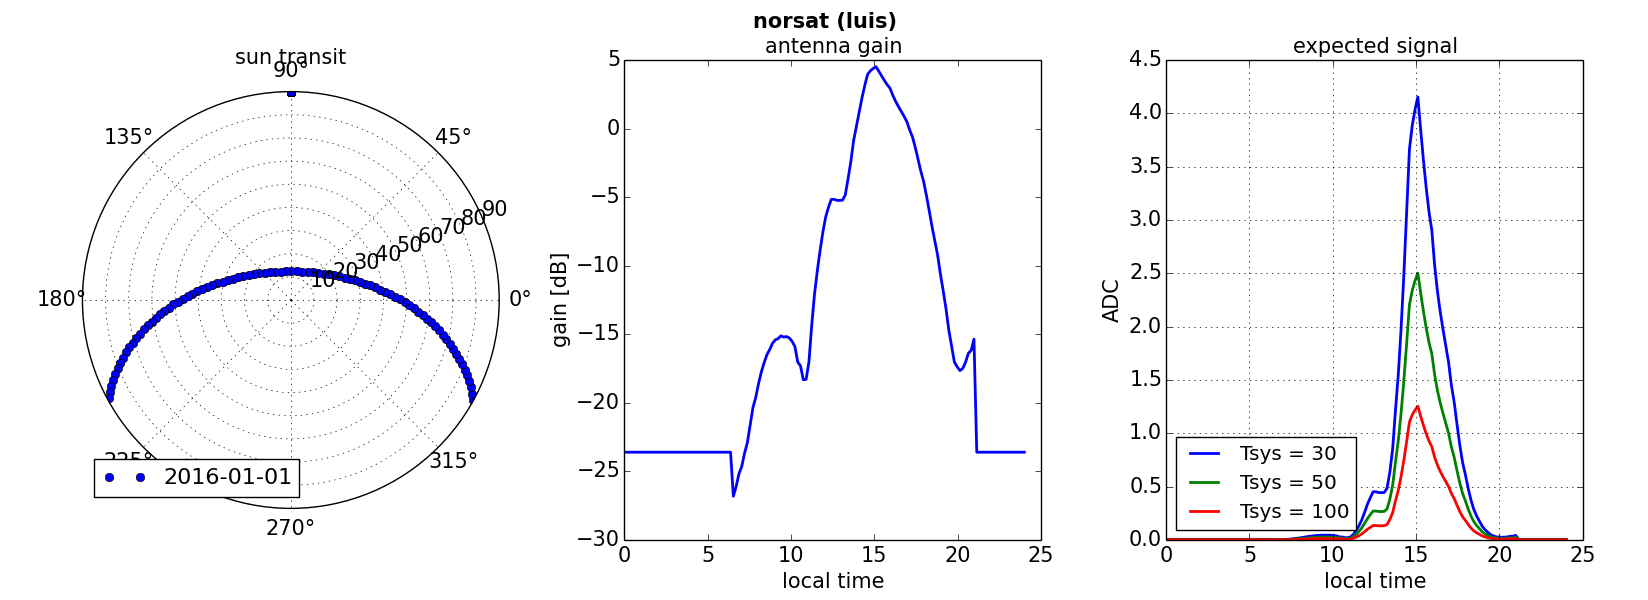
\includegraphics[width=0.7\linewidth]{expluis20160101.png}}\\
  \caption{Left: quiet sun spectrum, Right: varying component spectrum}
  \label{fig:spectra}
\end{figure}

\begin{figure}[!ht]
  \centering
  \hspace*{-3ex}
  \subfigure{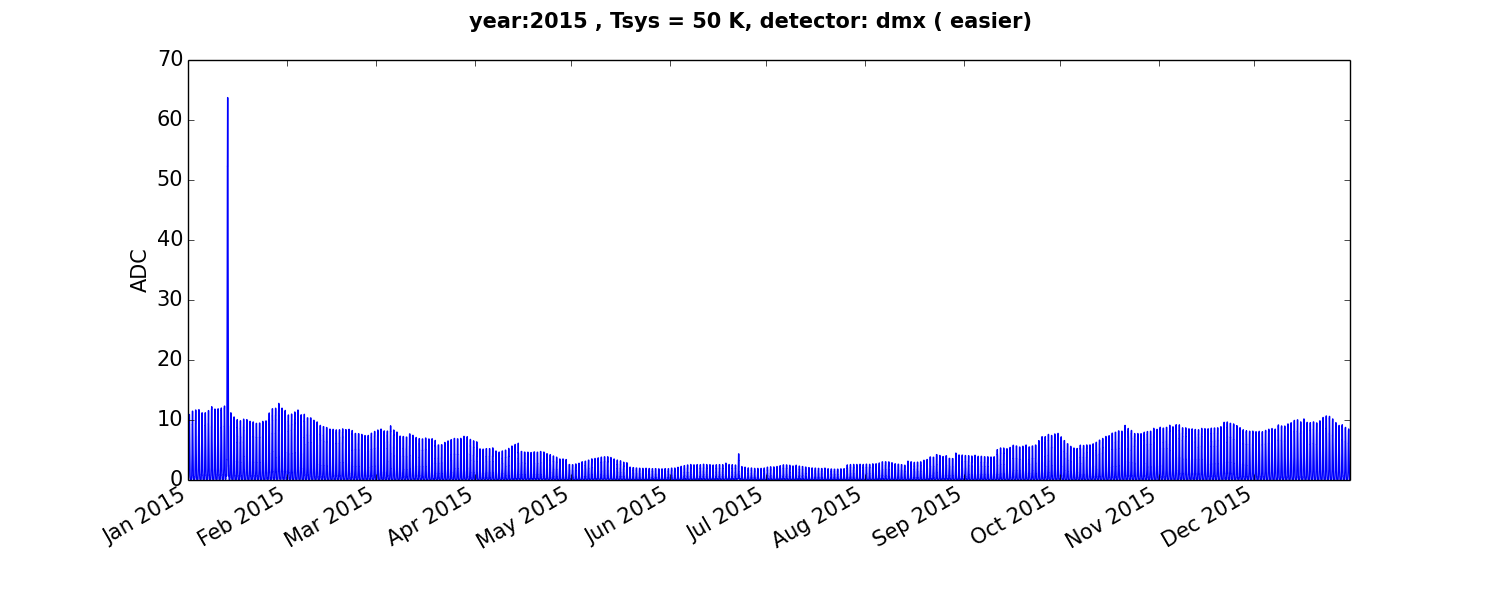
\includegraphics[width=0.7\linewidth]{year2015easier.png}}\\
  \subfigure{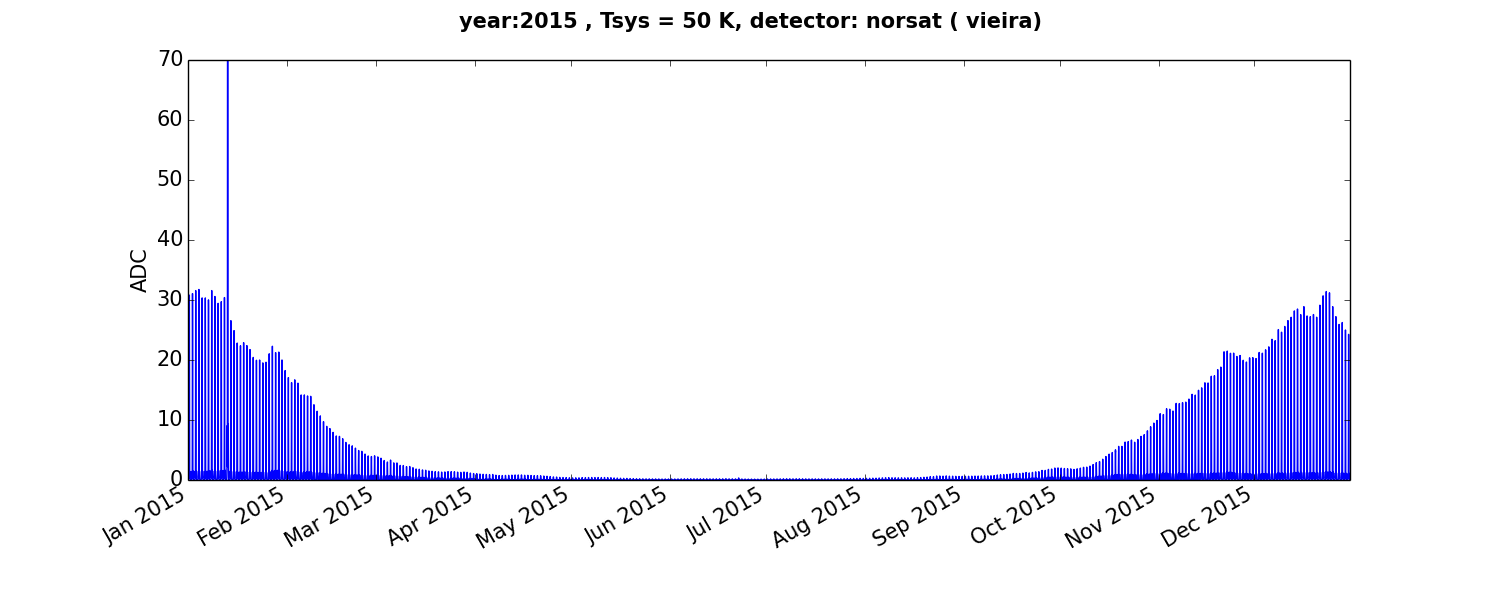
\includegraphics[width=0.7\linewidth]{year2015vieira.png}}\\
  \subfigure{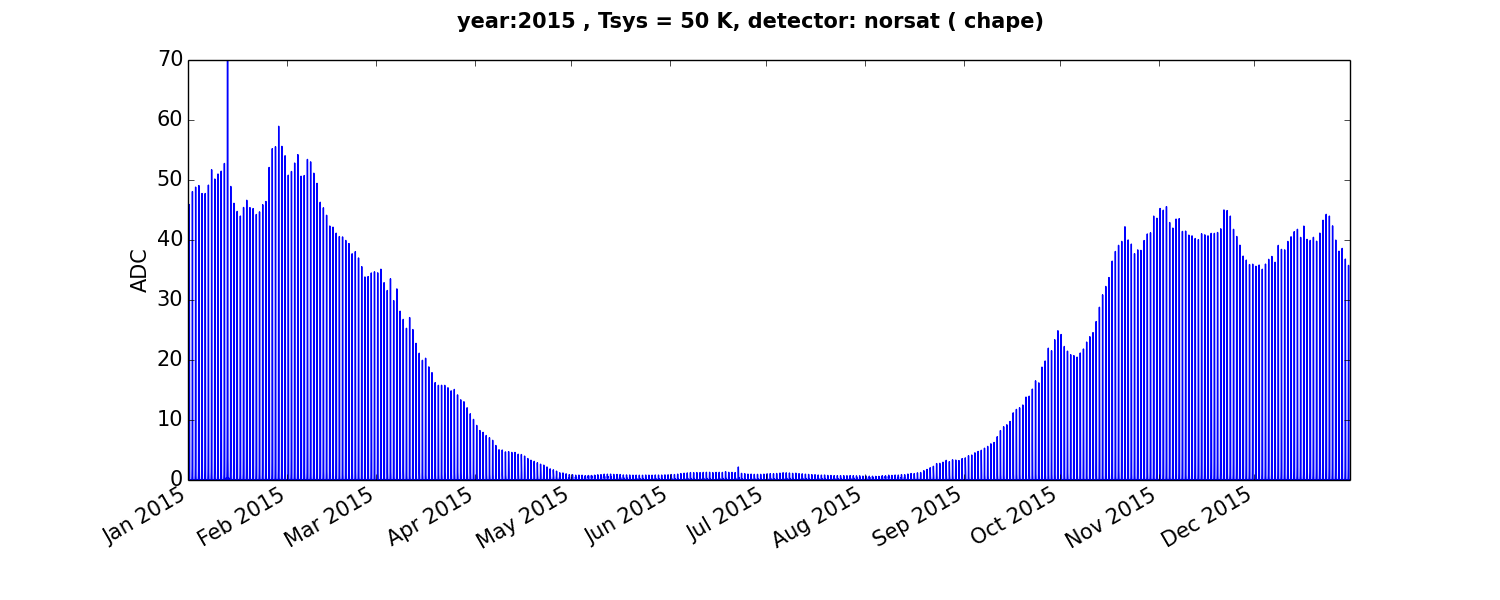
\includegraphics[width=0.7\linewidth]{year2015chape.png}}\\
  \subfigure{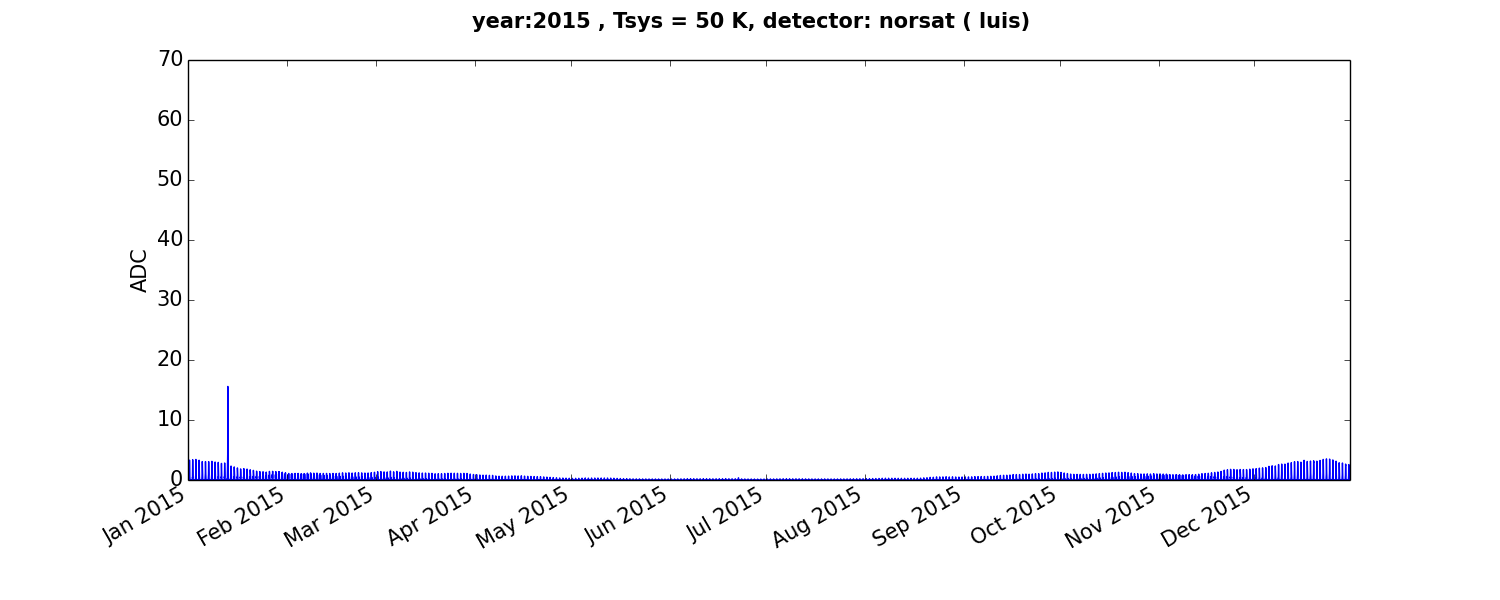
\includegraphics[width=0.7\linewidth]{year2015luis.png}}\\
  \caption{Left: quiet sun spectrum, Right: varying component spectrum}
  \label{fig:spectra}
\end{figure}


